% CSCI 7610 Graduate Technical Seminar paper
% Two-column layout following "Sample paper format.docx":
% US Letter, 1 in margins, Times, 14 pt title, 12 pt author block,
% 10 pt justified body, 9 pt references, Roman-numeral sections.
\documentclass[10pt,letterpaper,twocolumn]{article}

\usepackage[utf8]{inputenc}
\usepackage[T1]{fontenc}
\usepackage{newtxtext,newtxmath}
\usepackage[letterpaper,margin=1in,columnsep=0.3in]{geometry}
\usepackage{graphicx}
\usepackage{booktabs}
\usepackage{tabularx}
\usepackage{array}
\usepackage{ragged2e}
\usepackage{xcolor}
\usepackage{titlesec}
\usepackage{caption}
\usepackage{enumitem}
\usepackage{stfloats}
\usepackage{microtype}
\usepackage{xurl}
\usepackage[hidelinks]{hyperref}
\urlstyle{same}

\pagestyle{empty}
\graphicspath{{figures/}}

% Section headings: "I.  Introduction", "A.  Subsection"
\titleformat{\section}{\large\bfseries}{\Roman{section}.}{0.6em}{}
\titlespacing*{\section}{0pt}{12pt plus 2pt minus 2pt}{6pt plus 1pt}
\titleformat{\subsection}{\normalsize\bfseries}{\Alph{subsection}.}{0.5em}{}
\titlespacing*{\subsection}{0pt}{8pt plus 2pt minus 1pt}{4pt plus 1pt}

% Captions: "Figure 1: ..." / "Table 1: ..."
\captionsetup{labelsep=colon,font=small,justification=centering}
\captionsetup[figure]{name=Figure}
\captionsetup[table]{position=top,skip=4pt}

% Wrapping table columns
\newcolumntype{L}{>{\RaggedRight\arraybackslash}X}
\newcolumntype{P}[1]{>{\RaggedRight\arraybackslash}p{#1}}
\renewcommand{\arraystretch}{1.15}

\begin{document}

\twocolumn[{%
\begin{center}
  {\fontsize{14}{17}\selectfont\bfseries
   Reproducing Defense-Grade Container Hardening\\
   with Open-Source Tooling\par}
  \vspace{14pt}
  {\fontsize{12}{14.5}\selectfont
   Michael Ford\\
   Department of Computer Science\\
   Georgia Southern University\\
   Savannah, GA, USA\\
   mf17903@georgiasouthern.edu\par}
  \vspace{20pt}
\end{center}
}]

\noindent\textbf{\textit{Abstract---}}Federal supply-chain mandates tell software teams what a secure container pipeline must produce, but not how to build one. The Department of Defense's Iron Bank publishes its hardening recipes on Repo1, which raises a practical question: how close can an outside team get to Iron Bank's standard using only those public artifacts and open-source tools? This paper answers that question for the NGINX 1.30 web server. The upstream nginx:1.30 image was profiled with Trivy, Grype, and Syft, and Iron Bank's public Dockerfile, hardening manifest, and configuration were broken down into a catalog of 17 controls. The upstream image carries 151 packages, runs as root, and returns 318 Trivy findings and 294 Grype findings, almost none of them in NGINX itself and only 28 with a fix available. Iron Bank's controls turned out to sit at the build and supply-chain level: a minimal UBI 10 base, hash-pinned inputs, and a non-root user. TLS, security headers, and request limits are left to the consuming program. An independent build reproduces 13 of the 17 controls, 10 of them confirmed in the built image. The hardened image is 22\% smaller, carries 32\% fewer packages, and has no Critical-rated or fixable vulnerability findings in Grype, against 25 and 109 in the upstream image scanned on the same day. Trivy could not score the hardened image because its database has no RHEL 10 coverage. A variant that stops at Iron Bank's recipe already removes nearly all Critical and High CVEs, while package removal accounts for the size reduction. Grype also misreported NGINX's own vulnerabilities, because the SBOM labels the nginx.org package as Red Hat's build. The remaining gap lies not in the recipe, which is fully readable, but in the process behind it, since the re-hardened base image, the vulnerability review, and the accredited signing chain all sit behind authenticated access.

\medskip
\noindent\textbf{\textit{Keywords:}} \textit{container hardening, software supply chain, Iron Bank, NGINX, SBOM, DevSecOps.}

% ---------------------------------------------------------------------
\section{Introduction}

The United States' adversaries are developing their military capabilities at an alarming rate, and the U.S. Department of Defense (DoD) has committed to bolstering its own. The DoD, particularly the United States Air Force (USAF), depends on a growing portfolio of software systems for logistics, sustainment, and mission planning, all in service of shorter delivery timelines, lower cost, and a preserved warfighting advantage. To sustain that portfolio, the Air Force operates a network of internal software factories alongside an array of contractor developers. Every piece of technology fielded through those pipelines expands the attack surface that adversaries can probe for vulnerabilities.

Securing these pipelines requires rigorous hardening of foundational open-source components before they reach operational environments. Within Platform One, Iron Bank addresses this challenge by curating and hardening container images of widely deployed open-source components, such as the NGINX web server, to serve as trusted baselines for software factories. This paper conducts a comparative empirical analysis between the upstream nginx:1.30 image on Docker Hub and Iron Bank's publicly documented hardened 1.30 build. The real question this paper answers is how close an outside team can get to that defense-grade standard using only public artifacts and open-source tooling. By analyzing differences across their Dockerfiles, entrypoint scripts, hardening manifests, and runtime configurations, this study measures the reduction in attack surface an independent hardening pipeline can achieve and the trade-offs that come with it.

The need for rigorous supply chain security appears in recent incidents. The 2020 SolarWinds Orion breach demonstrated how a compromised build environment can distribute malicious code to thousands of government and enterprise networks at once. A year later, the Log4Shell vulnerability exposed the cascading risks of a single flaw in a ubiquitous open-source dependency. Most recently, the 2024 XZ Utils backdoor revealed details consistent with nation-state operations targeting foundational Linux utilities, proving that even well-scrutinized open-source projects are vulnerable to multi-year social engineering and sophisticated supply chain manipulation.

The federal government has responded to this class of threat over time, with mandates and industry frameworks such as Executive Order 14028, the NIST Secure Software Development Framework (SSDF), and Supply-chain Levels for Software Artifacts (SLSA) establishing baseline security requirements. However, a critical gap remains. These policies define required security outcomes but leave the technical implementation to practitioners. Iron Bank operates a working example of what closing that gap looks like, and it publishes its hardening manifests, Dockerfiles, and configurations as public artifacts on Repo1. But having access to those artifacts is not the same as being able to reproduce comparable results with them, especially from outside the DoD contractor pipeline. This research addresses that reproducibility question by building an independent, open-source hardening pipeline for the NGINX container image and measuring how close it can come to the Iron Bank benchmark. The resulting implementation guide transforms high-level policy into concrete engineering steps and answers a broader question about how accessible defense-grade OSS hardening actually is to teams working outside the DoD contractor pipeline.

% ---------------------------------------------------------------------
\section{Previous Works}

This research draws on four related areas: the growing threat to the software supply chain, the Department of Defense's use of open-source software, the rules and frameworks that govern secure software, and the technical methods used to harden containers.

Attacks on open-source software have grown more frequent and more sophisticated over the past five years. Yang, Lee, and McDonald (2022) describe the 2020 SolarWinds Orion breach as a turning point, showing how attackers who compromise a trusted build system can push malicious code to thousands of downstream users at once. The Log4Shell vulnerability that followed, tracked by CISA as CVE-2021-44228, showed how a single flaw in a widely used component can put nearly every Java-based system at risk. The 2024 XZ Utils backdoor (CVE-2024-3094), discovered by Freund, went further still. It revealed a multi-year social engineering effort against a single maintainer, with tradecraft consistent with nation-state operations, aimed at planting a hidden vulnerability in a core Linux utility. Imtiaz, Khanom, and Williams (2023) add to this picture by showing that open-source projects release security fixes at highly variable rates across ecosystems, meaning defense consumers cannot assume uniform upstream responsiveness. Together, these cases show that scanning code for known problems is not enough. Defenders also need to harden the software itself and track where each piece comes from.

The Department of Defense has responded to these threats by changing how it consumes open-source software. The DoD Enterprise DevSecOps Reference Design and Platform One documentation describe a central approach in which securing open-source components is treated as a national security issue rather than something each program handles on its own. Iron Bank sits at the center of this approach as the DoD's official source of signed, hardened container images, and Anchore's case study on Platform One explains how every component must pass continuous security checks before it can be used. However, the DoD's public documents describe the overall process without giving the step-by-step technical instructions an outside team, or a new software factory, would need to build a similar pipeline on its own.

A growing set of federal rules and industry frameworks now shapes how secure software should be built and delivered. Executive Order 14028 (2021) pushed the federal government toward zero-trust security, and its ideas were later turned into specific requirements in NIST SP 800-218, the Secure Software Development Framework, and NIST SP 800-161r1. Two industry efforts add to these federal standards: the OpenSSF Supply-chain Levels for Software Artifacts (SLSA v1.0) and CISA's Minimum Elements for a Software Bill of Materials, both of which define how to prove where software comes from and confirm it has not been tampered with. More recent actions, including Executive Order 14144 and the January 2026 OMB M-26-05 directive, show that this issue remains a top federal priority. All of these frameworks share one important feature. They say what a secure pipeline should produce, such as an SBOM or proof of provenance, but they leave the actual technical steps up to the people building the systems. That creates a gap between what the rules require and how teams should actually meet those requirements in practice.

Academic researchers have studied many of the technical methods used to harden containers and the systems that run them. Russell and Dev (2024) demonstrate how a centralized logging approach paired with open-source tools can surface and mitigate common Kubernetes misconfigurations before attackers exploit them. Cesarano and Natella (2025) introduce KubeFence, which filters Kubernetes API requests at a granularity beyond what native RBAC can enforce, shrinking the control plane's exposed attack surface. Morić, Dakić, and Čavala (2025) combine a theoretical threat model with a practical compliance assessment across both the control plane and the workloads running on it. This research supports the value of strong runtime controls, but it focuses on Kubernetes broadly, not on defense software pipelines or the specific frameworks that govern them. Lamb and Zacchiroli (2022) approach the problem from the build side, arguing that trusting source code is not the same as trusting the executables built from it. In their model, that trust comes only from showing that multiple, independent builders produce bit-for-bit identical results from the same pinned sources. Pinning every input by hash, as a hardening manifest does, controls what goes into a build but not what comes out of it, which leaves a consumer relying on whoever ran the build.

Despite the robust body of work, a gap remains. No public study takes a specific open-source component used by defense software factories, hardens it end-to-end using only open tools, produces the SBOM and provenance records that current federal rules require, and then compares the result against a public DoD hardening standard. Instead of simply hardening NGINX, the result quantifies the accessibility gap that outside teams face when reproducing DoD-grade container security from public artifacts alone. That accessibility question matters because software factories continue to proliferate across organizations, each needing trustworthy baselines independent of Iron Bank. This paper aims to fill that gap by carrying out and documenting this process on the NGINX 1.30 container image.

% ---------------------------------------------------------------------
\section{Methodology}

To achieve the goal of hardening open-source software with open-source tools, the study requires a defined methodology that any outside organization can successfully reproduce. The methodology proceeds in five stages: setting up the assessment environment and toolchain, capturing a baseline profile of the upstream nginx:1.30 image, extracting Iron Bank's publicly documented hardening controls into a reference catalog, applying those controls to an independent build of the same component, and evaluating the hardened result against the reference benchmark. This methodology borrows from established penetration testing practice by treating attack surface identification as the first-order measurement. This will involve examining installed packages, exposed ports, running processes, and default configuration files that the baseline container carries, as well as assessing each element for potential removal, restriction, or replacement in the hardened build.

The assessment environment is a Kali Linux virtual machine running under a KVM hypervisor. Kali serves as the analyst workstation and provides a stable, isolated container host for both the baseline and hardened images. All scanning, building, and comparison work happens inside this guest, keeping the study self-contained and reproducible from a single system image. The toolchain layers on top of Docker and consists entirely of freely available, open-source utilities. Trivy and Grype provide vulnerability scanning against two independent CVE databases so that findings can be cross-checked rather than trusted from a single source. Syft generates a Software Bill of Materials in CycloneDX and SPDX formats to inventory every component present in an image. docker-bench-security applies the CIS Docker Benchmark to configuration hygiene, and dive breaks down the layer-by-layer contents of an image so wasted space and unnecessary files become visible. Cosign, from the Sigstore project, produces cryptographic signatures and provenance attestations that satisfy the artifact requirements defined in NIST SP 800-218 and SLSA v1.0. Every tool in this list is publicly obtainable and runs on inexpensive hardware. In addition, it produces machine-readable output in JSON or a widely used SBOM format. This should allow for greater accessibility and flexibility.

With the toolchain in place, the study captures a baseline profile of the upstream nginx:1.30 image pulled directly from Docker Hub. Baseline capture is a procedural step, not a hardening step. Its purpose is to record the starting state in enough detail that any later change can be attributed to the hardening work rather than to environmental drift. Each pulled image is recorded by its full SHA-256 digest at the moment of scan so that identical bytes can be re-examined later. The metric categories captured for the baseline include image size, layer count, installed package count, SBOM component count, exposed ports, container user context, presence of a shell and package manager, CVE counts by severity from both scanners, and the response headers returned by a running instance of the container. All scan output is written to timestamped JSON files so the baseline snapshot is portable and simple to compare against later measurements.

Parallel to the baseline capture, the study builds a reference control catalog from Iron Bank's publicly documented artifacts. The source is the public GitLab repository at repo1.dso.mil, specifically the dsop/\allowbreak opensource/\allowbreak nginx/\allowbreak 1.30/\allowbreak nginx project. Four files carry the information that matters: the Dockerfile, the hardening\_manifest.yaml, the README, and the conf/nginx.conf. Each hardening decision embedded in those files is extracted and categorized. No authenticated access to Registry1 or the internal Vulnerability Assessment Tracker is used. This is intentional. Restricting the reference material to what is publicly reachable reinforces the accessibility question the study is designed to answer. The extracted controls fall into a small number of categories that structure the hardening work that follows. The categories in Table~1 were set before the artifacts were examined and are consistent with widely published hardening guidance, such as the CIS Docker Benchmark and the CIS NGINX Benchmark, while the Provenance category reflects the signed artifacts and SBOMs that NIST SP 800-218 treats as secure-development outputs.

\begin{table*}[tb]
\caption{Hardening controls by category, as anticipated before the Iron Bank artifacts were extracted (see Table~4 for what the artifacts contain).}
\label{tab:catalog}
\small
\begin{tabularx}{\textwidth}{@{}P{0.19\textwidth}LL@{}}
\toprule
\textbf{Hardening Category} & \textbf{Iron Bank Reference} & \textbf{Independent Reproduction} \\
\midrule
Base Image & Iron Bank-hardened UBI9 (Registry1) & Public redhat/ubi9, digest-pinned (Docker Hub) \\
User Context & Non-root user & Non-root user \\
Package Minimization & Minimal package set with cache cleanup & dnf install + clean, purge unused packages \\
Default File Removal & Removed nginx defaults and sample configs & RUN rm on default index, error pages, sample configs \\
TLS Configuration & TLS 1.2+, modern cipher suites & TLS 1.2+, modern cipher suites \\
Server Header & server\_tokens off & server\_tokens off \\
Security Headers & HSTS, X-Content-Type-Options, X-Frame-Options, CSP & Same set applied via add\_header directives \\
Resource Limits & Client body, timeout, and connection limits & Same limits applied \\
Provenance & Signed via Iron Bank build pipeline & Cosign keyless signing plus SBOM attestation \\
\bottomrule
\end{tabularx}
\end{table*}

The independent hardening pipeline mirrors this reference catalog category by category. Building the hardened image begins with a fresh Dockerfile that starts from Red Hat's public UBI 10 minimal image, pinned to a specific digest so that every rebuild starts from the same base. NGINX is installed on top of that base with only the packages the application requires, and any package manager caches are cleared in the same layer to avoid preserving them in the final image. A non-root user is created and the container's runtime USER instruction is set to that account. Default nginx files are removed and replaced with a hardened nginx.conf that turns off server token disclosure, restricts TLS to modern protocol versions and cipher suites, adds the standard set of security response headers, and imposes body size, connection, and timeout limits. Where practical, the shell and package manager are removed from the final image layer so that an attacker who reaches the container has nothing on hand to work with.

Because a hardened image that does not work is not hardened at all, the pipeline uses an iterate-scan-verify loop rather than a single-pass build. Each change to the Dockerfile or configuration triggers a rebuild, a rescan by every tool in the toolchain, and a functional check that confirms the container still serves an HTTP response. Deviations from the reference catalog are recorded with a short justification, either because a control does not apply to the upstream base or because reproducing it would require infrastructure the study cannot access. When the image reaches a stable state, Syft generates its SBOM and Cosign signs the image and produces a provenance attestation. All Dockerfiles, configuration files, build scripts, scan outputs, and produced artifacts are kept in a local git repository so that the exact state of the study at any point can be reconstructed.

Evaluation of the hardened artifact against the reference benchmark uses three categories of measurement. The primary measurement is the percentage of Iron Bank's documented hardening controls successfully replicated in the independent image, calculated by comparing the reference catalog against a control-by-control audit of the hardened build. Secondary measurements quantify the empirical effect of the hardening work: reduction in CVE counts by severity across both scanners, reduction in image size and layer count, reduction in installed package count, reduction in exposed ports and shell availability, and the presence of framework-compliance artifacts such as the SBOM and signed attestation. A third set of measurements records what the hardening work cost: any increase in Dockerfile complexity, any deviation from upstream functional parity, and any deployment flexibility given up to reach the hardened state. The study characterizes the gap between the independent build and the reference benchmark rather than passing or failing against a fixed threshold, because the research question asks how close outsiders can get, not whether they can achieve perfect parity.

Several factors could weaken the study's conclusions and warrant explicit acknowledgment. Iron Bank's internal scan reports are gated behind an authenticated Vulnerability Assessment Tracker, so the study compares the independent build against Iron Bank's documented hardening decisions rather than against Iron Bank's own scan output. Scanner-based measurement is itself a proxy for security posture. It catches known CVEs and misconfigurations but does not measure resistance to novel or maintainer-compromise attacks of the type demonstrated by the XZ Utils incident. Version drift between the upstream nginx:1.30 tag and the Iron Bank 1.30 build is possible at any given point, and the study mitigates this by pinning both images to specific digests at the moment of scan and by documenting those digests alongside every result. Some CVE deltas will reflect differences between the Debian base of upstream nginx and the Red Hat UBI base of the Iron Bank build rather than differences in hardening quality, so where possible the study normalizes comparisons by control category rather than by raw finding count. Finally, the study examines a single open-source component. Findings for NGINX establish a data point but do not by themselves generalize to more complex components such as databases, service meshes, or machine learning infrastructure. Extending the methodology to additional targets is left to future work.

% ---------------------------------------------------------------------
\section{Empirical Results}

This section reports the results of carrying out the methodology described in Section III. The study ran Stages 1 through 3 (environment setup, baseline capture, and reference extraction) on the Kali Linux virtual machine on September 18, 2026, and Stages 4 and 5 (the hardened build and its evaluation against the baseline and the reference catalog) on the same virtual machine on October 26, 2026. On October 28 and 29, both images were rescanned with the same vulnerability databases, and two variant builds were scanned alongside them, so that the comparisons in Tables~6 and~7 do not depend on database drift.

\subsection{Data Collection and Preprocessing}

Three data sources feed the results. The first is the upstream nginx:1.30 image pulled from Docker Hub on September 18, 2026, and recorded by its digest (sha256:f91bdb7a\ldots9676c45). It contains NGINX 1.30.5 on Debian 13.6 (``trixie''). The second is Iron Bank's public repository for the same component on Repo1, from which the Dockerfile, Dockerfile.arm64, hardening\_manifest.yaml, README.md, and conf/nginx.conf were downloaded without logging in. The manifest identifies the Iron Bank build as NGINX 1.30.4 on a UBI 10 minimal base, tag 10.2, so the Iron Bank build is one patch release behind upstream, and the manifest does not record why. The third source is the output of the scanning suite: Trivy 0.74.0, Grype 0.119.0 with a vulnerability database built the same morning, Syft in CycloneDX and SPDX formats, docker-bench-security 1.6.0, and a runtime probe that starts the container and records its response. The October 29 comparison scans used the same tool versions with databases downloaded that day.

Two preprocessing decisions shape the numbers. First, both scanners report one finding per package and vulnerability pair, so a CVE that affects both curl and libcurl is counted twice. The tables therefore report total findings, which is each scanner's headline number, alongside the count of unique CVE identifiers. Second, the scanners use different severity scales: Grype has a Negligible tier that Trivy does not. Severities are reported as each tool assigns them rather than forced onto a common scale.

Two tools did not produce usable baseline data. dive failed with a permission error because the scan script called it without sudo, so layer-efficiency data is not available. docker-bench-security evaluated every image on the virtual machine, including images left over from an earlier project, so only its NGINX-specific result is used: the image has no HEALTHCHECK instruction (CIS 4.6). Both problems were fixed for the hardened scans: dive ran with Docker access, and the hardened image passes the CIS 4.6 check (Section IV.F).

\subsection{Baseline Profile Results}

Table~2 summarizes the upstream image as it ships. The image is 169.5~MB across 7 layers and contains 151 Debian packages. It sets no USER instruction, so the NGINX master process starts as root. It includes two shells (bash and dash), a complete package manager (apt and dpkg), and curl. It also installs five optional NGINX modules (acme, geoip, image-filter, njs, and xslt) along with the image, XML, and GeoIP libraries they depend on, even though the stock configuration loads none of them. A running instance answers on port 80 with the default ``Welcome to nginx!'' page and a Server header that discloses the exact version, nginx/1.30.5. None of the four security headers listed in Table~1 is present.

\begin{table}[tb]
\caption{Baseline profile of the upstream nginx:1.30 image.}
\label{tab:baseline}
\small
\begin{tabularx}{\columnwidth}{@{}LP{0.44\columnwidth}@{}}
\toprule
\textbf{Metric} & \textbf{Upstream nginx:1.30} \\
\midrule
Digest & sha256:\allowbreak f91bdb7aee4cba26\ldots6c45 \\
NGINX version / base OS & 1.30.5 / Debian 13.6 \\
Image size & 169,475,103 bytes (169.5 MB) \\
Layer count & 7 \\
Installed packages (dpkg) & 151 \\
SBOM packages / file entries (Syft) & 152 / 3,227 \\
Exposed ports & 80/tcp \\
Runtime user & root (no USER instruction) \\
Shell present & Yes (bash, dash) \\
Package manager present & Yes (apt, dpkg) \\
Optional NGINX modules installed & 5 (none loaded by default) \\
Server header & nginx/1.30.5 \\
Security headers (HSTS, XCTO, XFO, CSP) & 0 of 4 \\
HEALTHCHECK instruction & None (CIS 4.6 warning) \\
\bottomrule
\end{tabularx}
\end{table}

Table~3 and Figure~1 give the vulnerability results. The two scanners largely agree on which vulnerabilities are present but not on how serious they are. Of the 179 distinct CVE identifiers reported by either tool, 164 (92\%) were reported by both. Their severity ratings, however, differ sharply. Trivy rates 4 findings Critical while Grype rates 25 Critical, because the two tools draw their ratings from different sources. This disagreement is the reason the methodology uses two scanners, since either tool alone would have given a noticeably different picture of the same image.

\begin{table}[tb]
\caption{Baseline vulnerability findings by severity.}
\label{tab:baseline-vulns}
\small
\setlength{\tabcolsep}{4pt}
\begin{tabularx}{\columnwidth}{@{}L*{4}{>{\centering\arraybackslash}p{0.15\columnwidth}}@{}}
\toprule
\textbf{Severity} & \textbf{Trivy findings} & \textbf{Trivy unique CVEs} & \textbf{Grype findings} & \textbf{Grype unique CVEs} \\
\midrule
Critical & 4 & 4 & 25 & 16 \\
High & 73 & 34 & 91 & 44 \\
Medium & 96 & 58 & 61 & 37 \\
Low & 118 & 70 & 10 & 7 \\
Negligible & n/a & n/a & 100 & 59 \\
Unknown & 27 & 11 & 7 & 3 \\
\midrule
\textbf{Total} & \textbf{318} & \textbf{177} & \textbf{294} & \textbf{166} \\
Fix available & 28 & --- & 28 & --- \\
\bottomrule
\end{tabularx}
\end{table}

\begin{figure}[tb]
\centering
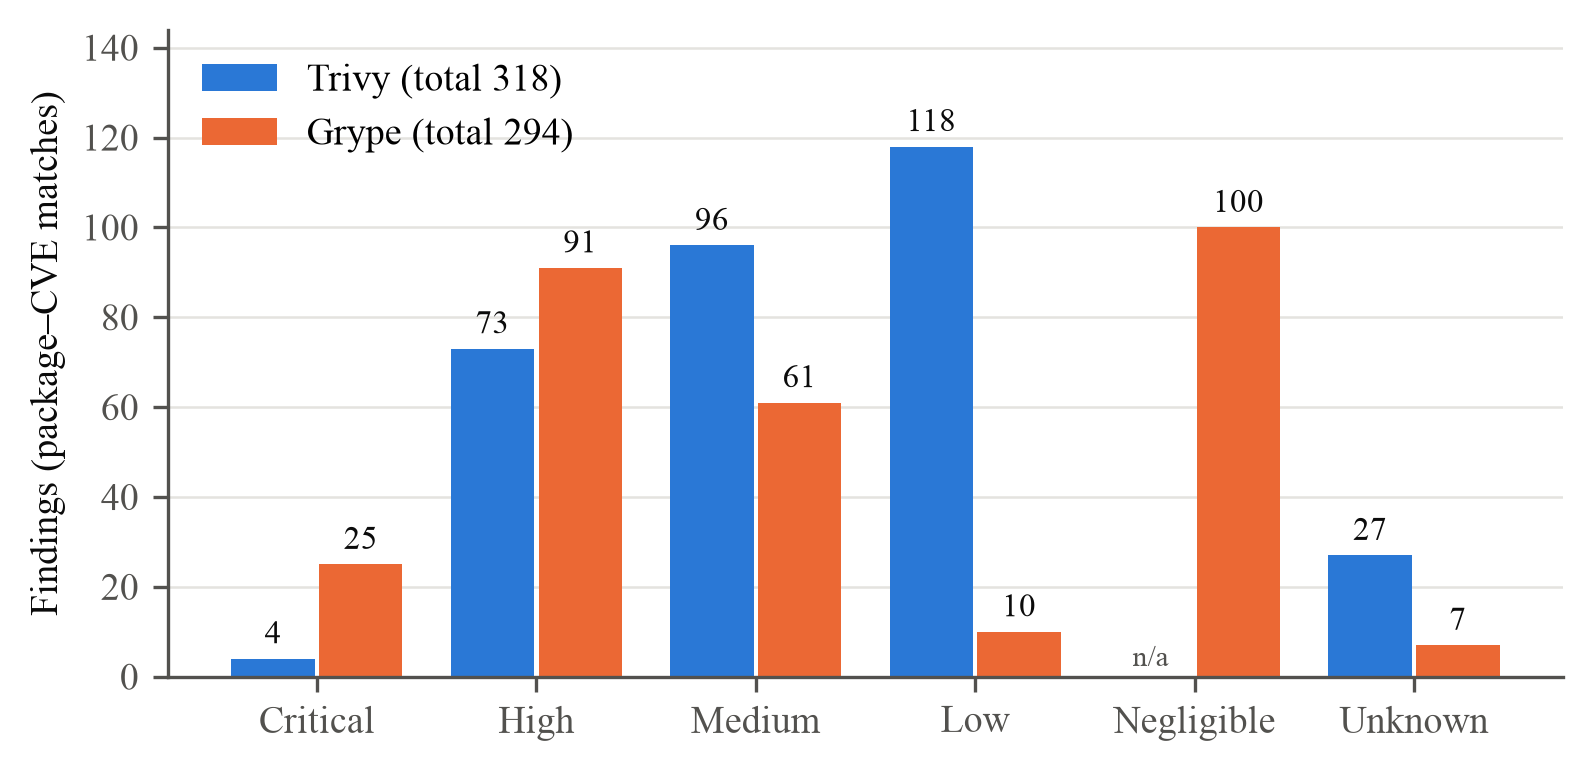
\includegraphics[width=\columnwidth]{fig_baseline_severity.png}
\caption{Baseline findings by severity, Trivy vs.\ Grype (nginx:1.30, September 18, 2026).}
\label{fig:baseline-severity}
\end{figure}

Patching alone cannot clean this image. On September 18, only 28 of Trivy's 318 findings (9\%) had a fixed package version available, and Grype classified 149 of its 294 findings as ones the distribution will not fix and 117 as not yet fixed. Fixes do arrive over time. When the same image was rescanned on October 29, Grype rated 109 of its 437 findings as fixable, but 328 (75\%) still had no fix. Rebuilding the same image after a fresh package update would therefore remove some findings but leave most of them, which leaves removing the packages that carry them as the main lever.

Figure~2 shows where the findings come from. The NGINX package itself accounts for none of Trivy's findings and for two old, low-rated findings in Grype (CVE-2009-4487 and CVE-2013-0337). The rest sit in the packages around it: shell and base utilities (107 findings, 34\%), curl and the libraries it depends on (72, 23\%), the libraries pulled in by the optional modules (64, 20\%), glibc (40, 13\%), and Perl (17, 5\%). curl and the optional-module libraries together account for 136 findings (43\%), and NGINX does not need either one to serve web content.

\begin{figure}[tb]
\centering
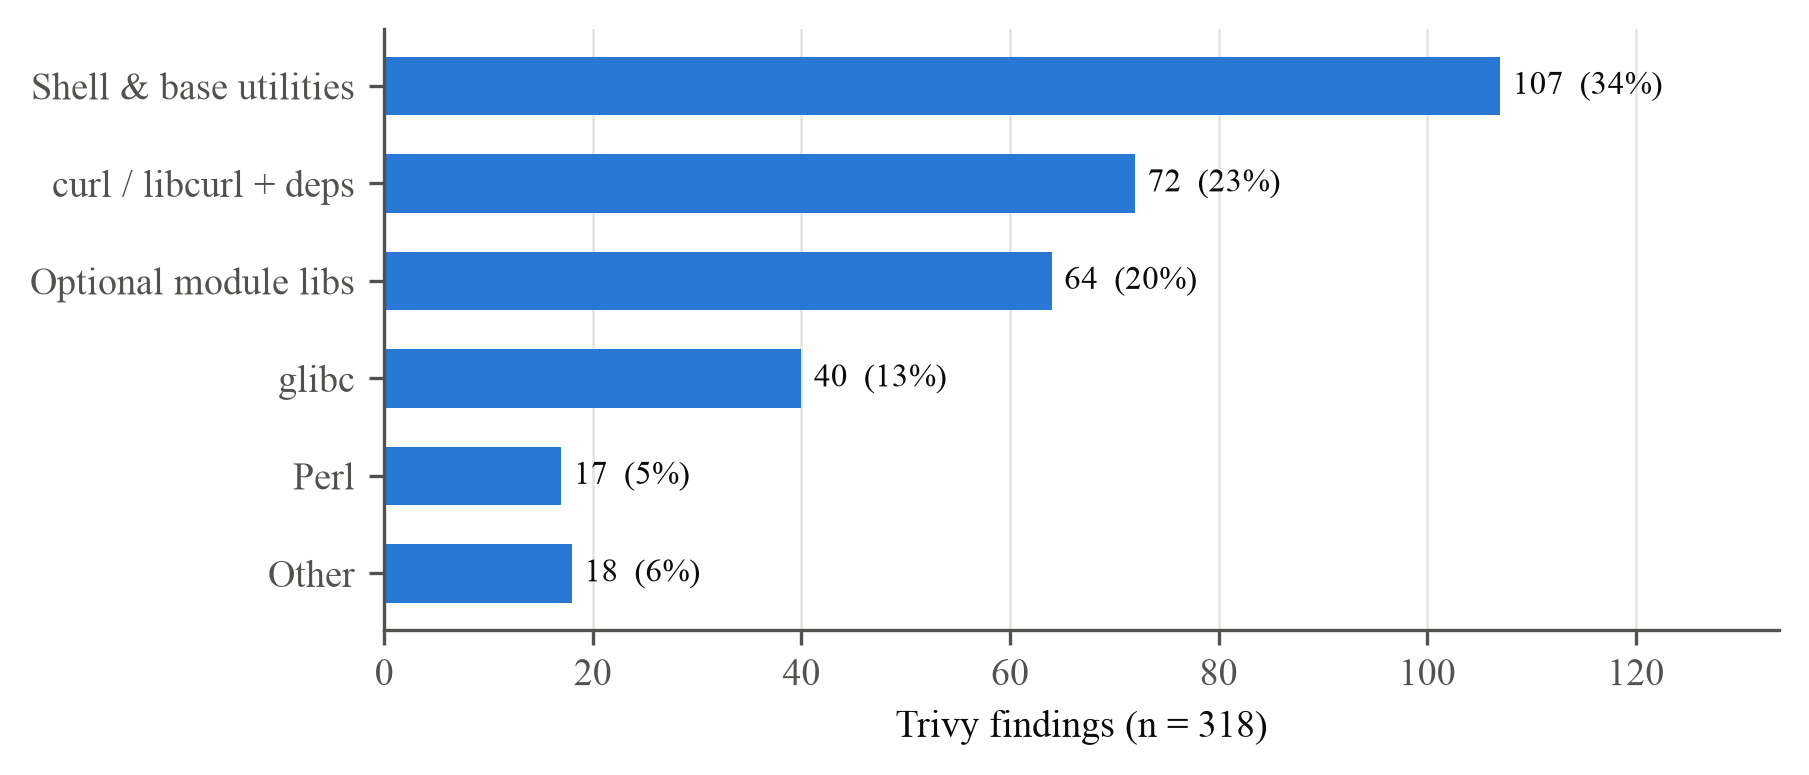
\includegraphics[width=\columnwidth]{fig_baseline_families.png}
\caption{Baseline Trivy findings grouped by the package family that carries them.}
\label{fig:baseline-families}
\end{figure}

\subsection{Reference Catalog Results}

Table~4 compares the controls anticipated in Table~1 with what Iron Bank's public artifacts actually contain. The extraction produced an unexpected result. Iron Bank's hardening is concentrated in how the image is built rather than in how NGINX is configured, and its nginx.conf is close to the stock NGINX configuration. It does not set server\_tokens off, adds no security headers, sets no request-size or timeout limits beyond the defaults, and does not configure TLS. Port 8443 is declared with a plain listen directive, so it serves unencrypted HTTP, and the HTTPS server block is commented out. The image is built as a hardened base that each consuming program configures for its own use, and the README supports this reading by showing consumers how to add their own content on top of it.

\begin{table*}[tb]
\caption{Anticipated controls (Table~1) compared with Iron Bank's public artifacts.}
\label{tab:anticipated-vs-found}
\small
\begin{tabularx}{\textwidth}{@{}P{0.16\textwidth}P{0.2\textwidth}LP{0.15\textwidth}@{}}
\toprule
\textbf{Category} & \textbf{Anticipated (Table 1)} & \textbf{Found in Iron Bank artifacts} & \textbf{Status} \\
\midrule
Base Image & Iron Bank-hardened UBI9 & Iron Bank-hardened UBI 10 minimal, tag 10.2 (Registry1, login required) & Present (different version) \\
User Context & Non-root user & USER nginx; root used only during the build & Present \\
Package Minimization & Minimal set with cache cleanup & Minimal base and caches removed, but dnf, gettext, and the versionlock plugin are added and kept & Partial \\
Default File Removal & Defaults and samples removed & conf.d/default.conf removed; packaged HTML directory copied into /etc/nginx and served & Partial \\
TLS Configuration & TLS 1.2+, modern ciphers & Not configured; port 8443 serves plain HTTP & Absent \\
Server Header & server\_tokens off & Not set, so the version is disclosed & Absent \\
Security Headers & HSTS, XCTO, XFO, CSP & None & Absent \\
Resource Limits & Body, timeout, connection limits & Defaults only (1024 worker connections, 65 s keepalive) & Absent \\
Provenance & Signed via Iron Bank pipeline & Inputs pinned by SHA-256 and RPM signature checked; image signing happens inside the pipeline and is not visible & Partial (inputs only) \\
\bottomrule
\end{tabularx}
\end{table*}

The build-level controls are substantial. The Dockerfile starts from Iron Bank's own re-hardened UBI 10 minimal image rather than the UBI 9 base that Table~1 assumed. Every external input is listed in hardening\_manifest.yaml with a download URL and a SHA-256 hash, and the NGINX signing key is imported so the RPM's signature is checked on install. The build applies all operating-system updates, installs NGINX from the official nginx.org RPM, locks its version, and clears the package caches. Runtime directories are handed to the unprivileged nginx user, write permission for other users is removed from the configuration and entrypoint scripts, logs are sent to standard output, the default server configuration is deleted, and the container switches to USER nginx and listens only on the unprivileged ports 8080 and 8443. An arm64 Dockerfile is kept in step with the x86\_64 one.

Control identification followed a bottom-up extraction procedure rather than a predefined checklist. Each of the four Iron Bank files was read line by line, and every discrete security intervention was recorded as a candidate control. For the Dockerfile, each directive that altered the runtime posture of the resulting image was treated as a candidate: base image selection, user context changes, individual package install or removal operations, file deletions, and configuration overlays. For the hardening\_manifest.yaml, each declaration that constrained the build or carried a security assertion was recorded, including the base image lineage, declared external resources with their validation hashes, and any CVE justifications, although the public manifest contains none. For the nginx.conf, each directive that altered the server's exposed surface or protocol behavior was recorded, including header suppression, response-header additions, TLS protocol and cipher restrictions, and connection and body limits. In Iron Bank's configuration, the only directives of this kind were the two unprivileged listen ports. The README contributed context rather than new controls and was used to confirm the intent behind decisions already extracted from the other three files. One control, pipeline signing with continuous scanning and CVE review, comes from Iron Bank's public documentation rather than from the four files, because the process it describes is not visible in them. Candidate controls were then grouped into categories by shared security outcome rather than by syntactic proximity. Where two syntactic steps produced a single outcome, they were merged into one control. For example, importing the NGINX signing key into both rpm and rpmkeys was treated as a single signature-verification control, because neither import serves a purpose without the signature check it enables. Where two steps produced distinct outcomes, they remained separate controls, even when they appeared on adjacent lines. The operating-system update and the package-cache cleanup that follows it, for instance, are recorded separately, because one changes which package versions ship and the other removes stored files. This procedure yielded the 17 controls listed in Table~5. A different researcher applying a stricter extraction rule would likely identify more controls, and one applying a looser rule would likely identify fewer; the categorization chosen here prioritizes a one-to-one correspondence between each listed control and a verifiable measurement that the hardened image can be judged against.

Table~5 lists the 17 controls extracted from these artifacts and whether each can be reproduced from public inputs. One part of the build could not be examined. The Dockerfile copies a scripts/ directory into the image as entrypoint scripts. Their names (IPv6 listening, template substitution, and worker tuning) appear in the Dockerfile, but the reference fetch retrieved only the six top-level files, so their contents were not reviewed. The lab evidence behind each entry in the table's last column is described in Section IV.F.

\begin{table}[tb]
\caption{Controls extracted from Iron Bank's public artifacts and their coverage in the independent build. Type: S = security, O = operational. Public = reproducible from public inputs. Built = replicated in the independent build (Equiv.\ = by equivalent means). Lab = verified in the built image (NP = set in the Dockerfile but not probed).}
\label{tab:controls}
\footnotesize
\setlength{\tabcolsep}{2.5pt}
\begin{tabularx}{\columnwidth}{@{}rL>{\centering\arraybackslash}p{0.07\columnwidth}*{3}{>{\centering\arraybackslash}p{0.105\columnwidth}}@{}}
\toprule
\textbf{\#} & \textbf{Iron Bank control} & \textbf{Type} & \textbf{Public} & \textbf{Built} & \textbf{Lab} \\
\midrule
1 & Minimal UBI 10 base image & S & Partial & Partial & Partial \\
2 & Inputs pinned by SHA-256 & S & Yes & Yes & Yes \\
3 & RPM signature verification & S & Yes & Yes & Yes \\
4 & OS updates at build time & S & Yes & Yes & Yes \\
5 & nginx.org RPM, version-locked & S & Yes & Equiv. & Yes \\
6 & Package cache cleanup & S & Yes & Yes & Yes \\
7 & Non-root runtime user & S & Yes & Yes & Yes \\
8 & Unprivileged ports 8080/8443 & S & Yes & Yes & Yes \\
9 & Runtime dirs owned by nginx & S & Yes & Yes & Indir. \\
10 & Others' write permission removed & S & Yes & Yes & NP \\
11 & Logs sent to stdout/stderr & O & Yes & Yes & Yes \\
12 & Default server config removed & S & Yes & Yes & Yes \\
13 & Graceful stop signal (SIGQUIT) & O & Yes & Yes & NP \\
14 & OCI metadata labels & O & Yes & Yes & NP \\
15 & arm64 build kept in step & O & Yes & No & --- \\
16 & Entrypoint scripts & O & Unk. & No & --- \\
17 & Pipeline signing, scanning, CVE review & S & No & Partial & Partial \\
\midrule
 & \textbf{Replicated / confirmed in lab} & & & \textbf{13} & \textbf{10} \\
\bottomrule
\end{tabularx}
\end{table}

\subsection{Hardened Image Results}

The independent build follows the Iron Bank recipe step for step wherever the inputs are public, and then adds the configuration controls that Table~1 anticipated. It starts from Red Hat's public UBI 10 minimal image, tag 10.2, which requires no login. It downloads the same NGINX 1.30.4 RPM and signing key listed in Iron Bank's manifest and refuses to build if either SHA-256 hash differs. The hardened nginx.conf turns off version disclosure, redirects plain HTTP to HTTPS, limits TLS to versions 1.2 and 1.3 with forward-secret ciphers, and adds the HSTS, X-Content-Type-Options, X-Frame-Options, Content-Security-Policy, and Referrer-Policy headers. It also caps request bodies at 1~MB, sets 10-second client timeouts, and limits connections and request rates per client address. Beyond the reference, the build strips setuid and setgid bits (CIS 4.8), adds a HEALTHCHECK (CIS 4.6), keeps configuration files owned by root so the running process cannot change them, and, in the same build step as the installation, removes dnf, microdnf, Python, and the other packages that dnf pulled in, keeping only those that the NGINX package itself requires, such as systemd and libxcrypt. Because the nginx.org RPM contains no optional modules, the five modules and their libraries from Figure~2 are not installed at all.

Table~6 places the two images side by side. Values for both images come from running the same scanning suite on October 29, 2026, with the same vulnerability databases, and are computed with the same script used for the baseline. The September 18 profile in Tables~2 and~3 remains the record of the image as it was pulled. Rescanning the same upstream bytes five weeks later raised Grype's count from 294 to 437 findings and its fixable count from 28 to 109, while the hardened image moved only from 258 to 260 findings between October 26 and 29. A comparison against the September baseline would therefore have understated the reduction considerably.

\begin{table*}[t]
\caption{Upstream image compared with the independent hardened build, both scanned October 29, 2026. Medium, Low, and Negligible counts are not comparable across the Debian and Red Hat severity scales (Section IV.D).}
\label{tab:comparison}
\small
\begin{tabularx}{\textwidth}{@{}P{0.28\textwidth}P{0.23\textwidth}LP{0.17\textwidth}@{}}
\toprule
\textbf{Metric} & \textbf{Upstream nginx:1.30} & \textbf{Hardened build} & \textbf{Change} \\
\midrule
Image size (MB) & 169.5 & 132.1 & $-$22.1\% \\
Layer count & 7 & 9 & +2 \\
Installed packages & 151 & 102 & $-$32.5\% \\
SBOM packages (Syft) & 152 & 102 & $-$32.9\% \\
Trivy findings (C / H / M / L / U) & 522 (5 / 89 / 167 / 174 / 87) & n/a (reports 0: no RHEL 10 data) & n/a \\
Grype findings (C / H / M / L / N / U) & 437 (25 / 140 / 101 / 25 / 112 / 34) & 260 (0 / 48 / 117 / 95 / 0 / 0) & $-$40.5\% \\
Unique CVEs (Trivy / Grype) & 269 / 235 & n/a / 159 & Grype $-$32.3\% \\
Grype unique Critical + High CVEs & 81 & 12 & $-$85.2\% \\
Grype fixable findings & 109 & 0 & $-$100\% \\
Exposed ports & 80/tcp & 8080/tcp, 8443/tcp & 1 $\rightarrow$ 2 (both unprivileged) \\
Runtime user & root & nginx & Non-root \\
Shell present & Yes & Yes (bash; a no-shell build also works) & \\
Package manager present & Yes (apt, dpkg) & rpm only (dnf, microdnf removed) & \\
Server header & nginx/1.30.5 & nginx (version hidden) & \\
Security headers & 0 of 4 & 4 of 4, plus Referrer-Policy & \\
TLS versions accepted & None (HTTP only) & TLS 1.2, 1.3 (1.0, 1.1 refused) & \\
SBOM / signed attestation & SBOM only & SBOM, Cosign signature, signed SBOM attestation & \\
HEALTHCHECK (CIS 4.6) & None (warning) & Present (passes) & \\
\bottomrule
\end{tabularx}
\end{table*}

\begin{figure}[tb]
\centering
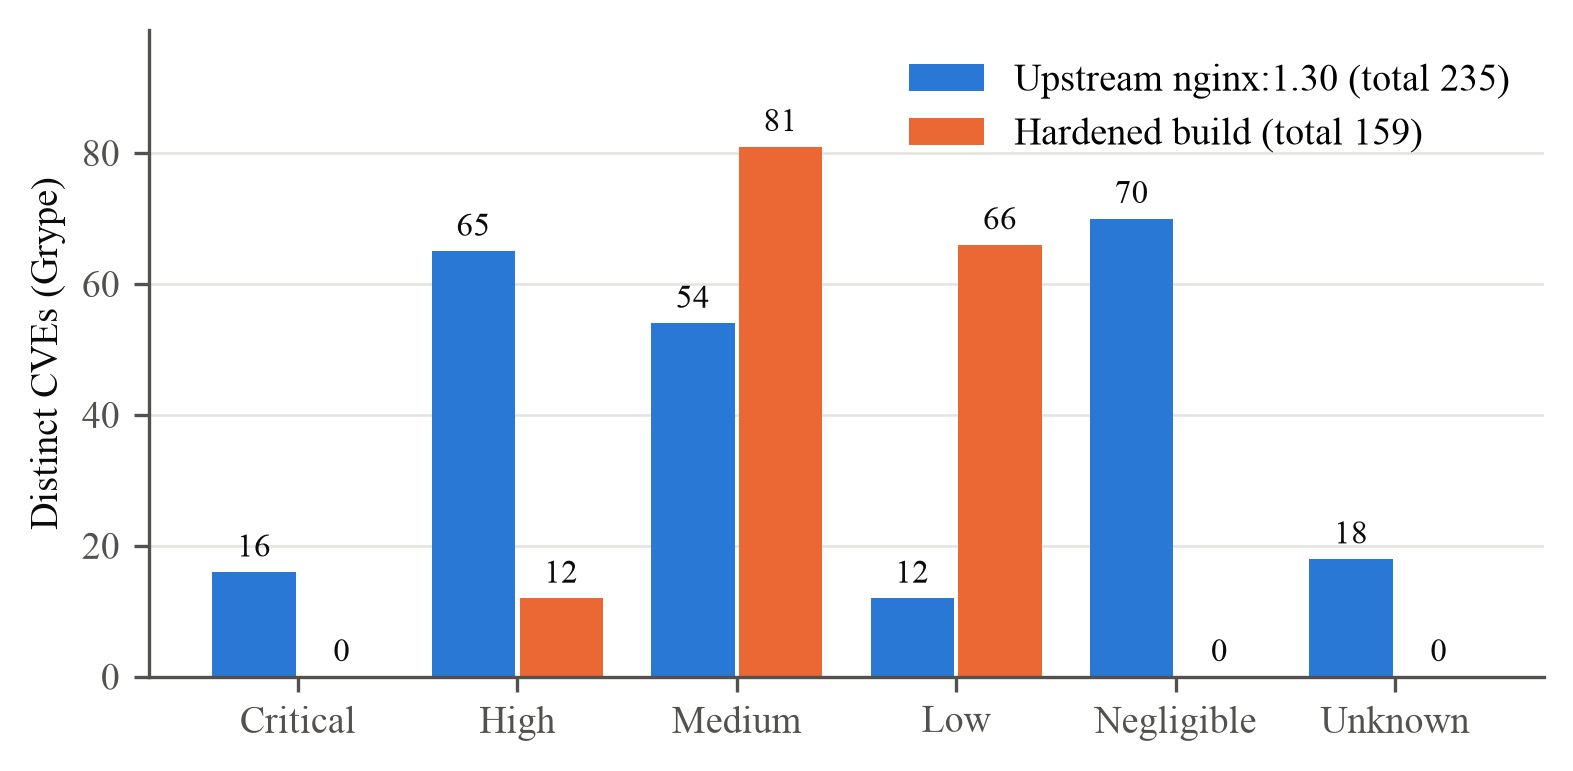
\includegraphics[width=\columnwidth]{fig_grype_before_after.png}
\caption{Distinct CVEs by Grype severity, upstream image vs.\ hardened build, both scanned October 29, 2026. Trivy is omitted because it cannot score RHEL 10 images.}
\label{fig:grype-before-after}
\end{figure}

Trivy reported zero findings for the hardened image, but that figure reflects a gap in Trivy's coverage rather than a clean image. Against Red Hat's public UBI 9 minimal image the same Trivy version reports 200 findings, but against the UBI 10 minimal base it reports none, and Trivy 0.76.1 behaves the same way. Grype finds CVEs in the same UBI 10 packages (curl, openssl-libs, util-linux), so Trivy's database simply has no RHEL 10 coverage yet. Table~6 therefore reports Trivy as n/a for the hardened image, and the comparison relies on Grype. A single-scanner pipeline built on Trivy alone would have reported a misleading 100\% reduction, which supports the methodology's decision to cross-check two scanners.

Grype's Medium and Low counts rose even as its totals fell, for two reasons. First, the two distributions rate severity differently. Debian places 70 of the baseline's CVEs in a Negligible tier that Red Hat does not use, while Red Hat rates comparable issues Low or Medium, so the Medium and Low rows rise. Only the Critical and High tiers and the fixable count compare cleanly across the two bases, and in those the change is large. Distinct Critical and High CVEs fell from 81 to 12, and fixable findings fell from 109 to none (Figure~3). Second, Grype reports each util-linux CVE once for each of its six subpackages, so 42 of the hardened image's 48 High findings are 7 util-linux CVEs counted six times. Every remaining finding is one that Red Hat lists as not yet fixed (256) or will not fix (4).

Image size depended not only on which packages were removed but also on where in the build they were removed. An earlier build removed the same packages in a separate RUN instruction and stayed at 235.1~MB, larger than upstream, because files deleted in a later layer still ship in the earlier one. Moving the removal into the installation step brought the image to 132.1~MB. dive still finds 37~MB of base-image files that later layers delete or replace (82\% efficiency), so flattening the image to one layer would shrink it further. Neither Dockerfile uses a multi-stage build. A builder stage that copies only NGINX and its runtime files into a minimal final stage would remove both the redundant base-image files and the need for in-layer package removal, but it would also depart from the package-managed layout that the comparison with Iron Bank depends on. The same layering effect appeared when the shell was removed. A variant build that removes bash in a later step serves HTTPS normally and has no shell at all, but at 145.7~MB it is larger than the final image, most likely because the removal runs in a separate layer and the package database it rewrites is stored a second time. A still earlier build, which removed only dnf and microdnf, isolates the effect of the rest: it carried 142 packages and 194 distinct CVEs, so removing Python and the remaining dnf dependencies took out another 40 packages and 37 CVEs.

Table~7 separates the two sources of improvement. A second variant followed the same Dockerfile but kept dnf and its dependencies, which approximates the image that Iron Bank's recipe produces from public inputs. It differs from Iron Bank's build in three ways: it does not add gettext or the versionlock plugin, it skips optional dependencies, and its operating-system update ran two days after the final build's. The recipe alone accounts for nearly all of the change in the severe tiers. Unique Critical and High CVEs fell from 81 to 13, and fixable findings fell to none, because the UBI 10 base and the build-time update replace Debian's packages with current Red Hat ones. The recipe also produced an image 31\% larger than upstream. Package-manager removal, which Iron Bank does not perform, contributed the size reduction, cutting the image from 221.6 to 132.1~MB, and removed 125 of the remaining findings, almost all of them Medium or Low. The configuration controls that the build adds beyond the recipe, such as TLS, security headers, and request limits, change no package and so do not appear in these counts at all.

\begin{table}[tb]
\caption{Contribution of Iron Bank's recipe and of package-manager removal (Grype, October 29, 2026).}
\label{tab:decomposition}
\small
\setlength{\tabcolsep}{4pt}
\begin{tabularx}{\columnwidth}{@{}L*{3}{>{\centering\arraybackslash}p{0.17\columnwidth}}@{}}
\toprule
\textbf{Metric} & \textbf{Upstream} & \textbf{Recipe only (dnf kept)} & \textbf{Final build} \\
\midrule
Image size (MB) & 169.5 & 221.6 & 132.1 \\
Installed packages & 151 & 149 & 102 \\
Findings & 437 & 385 & 260 \\
Unique CVEs & 235 & 196 & 159 \\
Unique Critical + High & 81 & 13 & 12 \\
Fixable findings & 109 & 0 & 0 \\
\bottomrule
\end{tabularx}
\end{table}

\subsection{NGINX Vulnerability Matching}

Neither scanner reports vulnerabilities in NGINX itself reliably. On October 29, Grype matched the nginx.org package against Red Hat's advisories for Red Hat's own NGINX build and reported 14 CVEs, two more than with the October 26 database. Checked against nginx.org's security advisories, 9 of them were fixed before 1.30.4 and do not apply. The other five do apply: CVE-2026-15176, CVE-2026-93479, and CVE-2026-97205, along with an HTTP/3 flaw, which this configuration does not enable, and a session-ticket flaw that its ssl\_session\_tickets off setting avoids. The newer database added those last two, which the October 26 scan had missed, but Grype still misses a second HTTP/3 flaw that affects 1.30.4. All six are fixed in NGINX 1.30.6. The upstream image's 1.30.5 is affected by five of them, yet Grype reported only two decades-old NGINX CVEs for it.

The SBOM explains the mismatch. Syft records the nginx.org package with the package URL \texttt{pkg:rpm/\allowbreak redhat/\allowbreak nginx@1.30.4-1.el10.ngx}, which identifies it as Red Hat's own build, and Grype then applies Red Hat's advisories to it. The same entry's CPE identifier is malformed, with the packager's e-mail address embedded in the vendor field. Any team that installs a vendor's RPM on a RHEL-family base inherits the same error, so scanner output for third-party packages has to be checked against the vendor's own advisories. It also means that an SBOM can satisfy a framework's format requirements while misidentifying the most security-relevant package in the image. Pinning the exact RPM listed in Iron Bank's manifest is what makes the build reproducible, and it is also what leaves it two patch releases behind.

\subsection{Evaluation Against the Benchmark}

The study evaluates the hardened build using the three categories of measurement defined in Section III.

\textbf{Primary measurement.} Of the 17 controls extracted from Iron Bank's public artifacts (Table~5), the independent build is designed to replicate 12 directly and one more, the version lock, by equivalent means, for 13 of 17 (76\%). Because this figure depends on how the controls are counted, it helps to separate them by purpose. Twelve of the 17 controls affect the image's security posture (controls 1--10, 12, and 17), and the build replicates 10 of them (83\%), with the other two partial. The remaining five are operational (log routing, the stop signal, metadata labels, the arm64 build, and the entrypoint scripts), and the build replicates three of these. Of the four controls outside the 13, two are partial: the base image is the public UBI 10 minimal image rather than Iron Bank's re-hardened copy, and pipeline signing is approximated with Cosign. Two are not replicated: the arm64 build was outside the study's scope, and the entrypoint scripts were not retrieved. Lab checks on the built image confirmed 10 of the 13: both SHA-256 checks and the RPM signature check passed, the update ran and left no fixable findings, the nginx.org RPM is the installed NGINX, no package-manager cache remains, the process runs as uid 998 and writes its PID file to the nginx-owned cache directory, it listens on 8080 and 8443, logs reach standard output, and the default server is gone. The other three (permission removal, the stop signal, and the labels) are set in the Dockerfile but were not separately probed. For the two partial controls, the base-image digest was recorded and the Cosign signature and SBOM attestation verified.

\textbf{Secondary measurements.} With both images scanned on the same day, Grype findings fell from 437 to 260 (40\%) and distinct CVEs from 235 to 159 (32\%), and the change is largest in the most severe tiers, where Critical and High findings fell from 165 to 48 (71\%), Critical findings from 25 to none, and fixable findings from 109 to none. Trivy could not score the hardened image (Section IV.D). Image size fell by 22\% and installed packages by 32\%. The number of exposed ports rises from one to two, matching Iron Bank, but both are unprivileged and the HTTP port only redirects to HTTPS. Both images now have an SBOM, but only the hardened image carries a signature and a signed SBOM attestation, both of which Cosign 3.1.3 verified against the build's public key. Table~1 anticipated keyless signing, but the build signs with a locally generated key pair and does not upload to Sigstore's public transparency log, because key-based signing works offline and can be repeated on the virtual machine without an external identity provider. The runtime probe confirms that dnf and microdnf are gone and only the low-level rpm tool remains. A shell is still present in the final image, but only because the scan suite's package inventory runs through one, which makes it a limitation of the measurement method rather than a hardening decision. NGINX itself does not need a shell. The variant build with bash removed served HTTPS normally, refused every attempt to start /bin/sh, and showed the same 260 Grype findings, since bash carried none. Removing the shell therefore takes tools away from an attacker without changing the scanner counts. An extended runtime probe also confirmed that the configuration controls added beyond the reference work as configured, not only that they appear in nginx.conf. A 2~MB request body was rejected with status 413, every method other than GET and HEAD was refused (403, or 405 for TRACE), a burst of 100 parallel requests produced 54 successes and 46 rate-limit rejections that NGINX logged, an idle connection was closed after the configured 10-second header timeout, and the Content-Security-Policy header was served as written. The per-address connection limit could not be isolated with a small test page and was not probed.

\textbf{Cost measurements.} The third set of measurements records what the hardening cost. The hardened Dockerfile has 47 non-comment lines, plus a 37-line package-removal script, against 41 in Iron Bank's, and the hardened nginx.conf has 66 non-comment lines against Iron Bank's 30. The image also departs from upstream behavior in several ways that a consuming team would notice. It listens on 8080 and 8443 instead of 80, will not start unless a TLS certificate is mounted, accepts only GET and HEAD requests with bodies up to 1~MB, drops the upstream entrypoint's environment-variable templating, and ships none of the optional modules. In addition, without a package manager, debugging tools cannot be installed into a running container. Each of these is a deliberate trade of flexibility for a smaller attack surface, and each is a setting a consuming team may need to relax. In the lab the image passed every functional check in every build (HTTP redirect, HTTPS response, all headers, TLS 1.1 refusal, and a non-root process), and its HEALTHCHECK clears the CIS 4.6 check that the upstream image fails.

\subsection{Discussion}

Most of the Iron Bank recipe was straightforward to reproduce, because Iron Bank builds from public inputs: the nginx.org RPM, the nginx.org signing key, and a UBI base that Red Hat also distributes publicly. The hardening\_manifest.yaml is, in effect, a reproducible bill of inputs, and an outside team can verify the same hashes. The configuration controls that Iron Bank leaves out were equally straightforward, since each is a documented NGINX directive.

However, a few controls needed workarounds. The base image had to be swapped for its public equivalent, and the version lock was replaced by removing the package manager, which makes the lock unnecessary. The runtime probe had to be rewritten because the hardened image no longer listens on port 80 and needs a mounted certificate, and because Cosign signs images in a registry, signing required a local registry on the virtual machine. Package removal also needed a dependency-aware script that runs in the same layer as the installation, because installing dnf pulls in libraries that NGINX itself requires.

What could not be reproduced is the process around the recipe. The contents of Iron Bank's re-hardened base image, its scan results, the justification written for each remaining CVE in the Vulnerability Assessment Tracker, its rebuild schedule, and the identity behind its signatures all require authenticated access. An outside team can produce a signature, but not one that a DoD program office has a reason to trust. This is the distinction Lamb and Zacchiroli (2022) draw between trusting source code and trusting the executables built from it. Both Dockerfiles apply operating-system updates at build time, so neither image can be rebuilt bit for bit, and an outside team has no way to check Iron Bank's published image against its public recipe.

Together, these results say something specific about accessibility. Technical hardening of a component like NGINX is within reach of an outside team using free tools on a single virtual machine, but assurance is not, because the independent review and accountable sign-off that make an Iron Bank image defense-grade cannot be copied from a repository. The extraction also carries a practical warning for teams that consume Iron Bank images. Its public configuration shows that TLS, security headers, and request limits are not included, so a program that deploys the image as-is still has to apply those controls itself.

The results also carry implications beyond this one component. For software factories that need a trusted baseline independent of Iron Bank, Table~7 suggests that most of the measurable benefit comes from the recipe itself, meaning a current minimal base, verified inputs, and build-time updates, which any team can adopt from public artifacts today. Package removal then pays for itself mainly in image size and in lower-severity findings. For policy, the findings show where current frameworks stop. NIST SP 800-218 and SLSA ask for an SBOM and provenance, and the hardened build produces both, yet its SBOM misidentifies the most important package in the image and its signature carries no identity that a program office would recognize. Producing the required artifacts is not the same as producing trustworthy ones, and guidance that names the artifacts without saying how they should be checked leaves that gap open.

% ---------------------------------------------------------------------
\section{Conclusion and Future Research}

This study asked how close an outside team can get to Iron Bank's defense-grade container hardening using only public artifacts and open-source tooling. For NGINX 1.30, an outside team can come close to the recipe and go further than the reference on configuration, but it cannot match the reference on assurance. Of the 17 controls extracted from Iron Bank's public artifacts, 14 are reproducible from public inputs and the independent build replicates 13 of them, 10 of which were confirmed in the built image. The build also adds TLS, security headers, request limits, and package-manager removal that the reference leaves to consumers. The hardened image is 22\% smaller, carries 32\% fewer packages, and has no Critical-rated or fixable vulnerability findings, against 25 Critical and 109 fixable in the upstream image scanned on the same day. Most of the reduction in severe findings comes from Iron Bank's recipe itself, which any outside team can follow, while package removal is what makes the image smaller than upstream. The baseline data also show why removal matters more than patching, since only 9\% of the upstream image's findings had a fix available when it was first scanned, three quarters still had none five weeks later, and 43\% sat in curl and optional-module libraries that NGINX does not need.

The study has several limits. It examines a single component, and its scanner findings are a proxy for security that does not measure resistance to an attack like the XZ Utils backdoor. The comparison is against Iron Bank's documented decisions rather than its own scan output, which requires authenticated access. The Iron Bank entrypoint scripts were not retrieved, and the Iron Bank build (1.30.4) is one patch release behind upstream (1.30.5). By the time of the hardened build, NGINX 1.30.6 had fixed six advisories that affect 1.30.4. Two measurement limits also emerged in the lab. Trivy's database has no RHEL 10 coverage, so the hardened image was scored by Grype alone, and neither scanner reported NGINX's own vulnerabilities accurately, because the SBOM misidentifies the nginx.org package, so NGINX findings were checked by hand against nginx.org's advisories. The study also covers only the image, not its runtime environment. Network policy, read-only root filesystems, dropped Linux capabilities, and orchestrator settings all affect a deployed container's attack surface but fall outside its scope.

Several extensions follow directly. The same pipeline can be applied to other components that Iron Bank publishes, such as databases and caches, to test whether the pattern of build-level hardening with consumer-level configuration holds. Running the pipeline on a schedule in a CI/CD system would show how quickly the CVE counts of both images drift as new vulnerabilities are published. A build on a smaller base, such as UBI micro or a distroless image, or a multi-stage build that copies only NGINX's runtime files into its final stage, would test how much further package removal can go. Finally, with authenticated Registry1 access, the Iron Bank image itself could be scanned with the same tools, turning the control comparison into a direct measurement comparison.

% ---------------------------------------------------------------------
\section*{References}

{\footnotesize
\begin{enumerate}[label=\arabic*.,leftmargin=*,itemsep=1pt,parsep=0pt,topsep=2pt]
\item Anchore, Inc. (n.d.). \textit{Grype: A vulnerability scanner for container images and filesystems}. \url{https://github.com/anchore/grype}
\item Anchore, Inc. (n.d.). \textit{Syft: CLI tool and library for generating a Software Bill of Materials from container images and filesystems}. \url{https://github.com/anchore/syft}
\item Anchore. (2021). \textit{Building a DevSecOps platform with the U.S. Air Force}. \url{https://anchore.com/blog/devsecops-platform-usaf/}
\item Aqua Security. (n.d.). \textit{Trivy: Comprehensive and versatile security scanner}. \url{https://github.com/aquasecurity/trivy}
\item Center for Internet Security. (n.d.-a). \textit{CIS Docker Benchmark}. \url{https://www.cisecurity.org/benchmark/docker}
\item Center for Internet Security. (n.d.-b). \textit{CIS NGINX Benchmark}. \url{https://www.cisecurity.org/benchmark/nginx}
\item Cesarano, C., \& Natella, R. (2025). KubeFence: Security hardening of the Kubernetes attack surface. In \textit{2025 55th Annual IEEE/IFIP International Conference on Dependable Systems and Networks (DSN)} (pp.~497--510). IEEE. \url{https://doi.org/10.1109/DSN64029.2025.00054}
\item Cybersecurity and Infrastructure Security Agency. (2021). \textit{Apache Log4j vulnerability guidance (CVE-2021-44228)}. U.S. Department of Homeland Security. \url{https://www.cisa.gov/news-events/news/apache-log4j-vulnerability-guidance}
\item Cybersecurity and Infrastructure Security Agency. (2024). \textit{Reported supply chain compromise affecting XZ Utils data compression library, CVE-2024-3094}. U.S. Department of Homeland Security. \url{https://www.cisa.gov/news-events/alerts/2024/03/29/reported-supply-chain-compromise-affecting-xz-utils-data-compression-library-cve-2024-3094}
\item Cybersecurity and Infrastructure Security Agency. (2025). \textit{Minimum elements for a Software Bill of Materials (SBOM)}. U.S. Department of Homeland Security. \url{https://www.cisa.gov/sbom}
\item Docker, Inc. (n.d.). \textit{Docker Bench for Security}. \url{https://github.com/docker/docker-bench-security}
\item Docker, Inc. (n.d.). \textit{nginx: Official build of Nginx} [Container image]. Docker Hub. \url{https://hub.docker.com/_/nginx}
\item Executive Order No. 14028, 3 C.F.R. 26633 (2021). Improving the nation's cybersecurity. \textit{Federal Register, 86}(93), 26633--26647.
\item Executive Order No. 14144, 3 C.F.R. 6755 (2025). Strengthening and promoting innovation in the nation's cybersecurity. \textit{Federal Register, 90}(11), 6755.
\item Freund, A. (2024, March 29). \textit{Backdoor in upstream xz/liblzma leading to ssh server compromise} [Mailing list post]. openwall.com. \url{https://www.openwall.com/lists/oss-security/2024/03/29/4}
\item Goodman, A. (n.d.). \textit{dive: A tool for exploring a docker image, layer contents, and discovering ways to shrink the size of your Docker/OCI image}. \url{https://github.com/wagoodman/dive}
\item Imtiaz, N., Khanom, A., \& Williams, L. (2023). Open or sneaky? Fast or slow? Light or heavy?: Investigating security releases of open source packages. \textit{IEEE Transactions on Software Engineering, 49}(4), 1540--1560. \url{https://doi.org/10.1109/TSE.2022.3181010}
\item Lamb, C., \& Zacchiroli, S. (2022). Reproducible builds: Increasing the integrity of software supply chains. \textit{IEEE Software, 39}(2), 62--70. \url{https://doi.org/10.1109/MS.2021.3073045}
\item Morić, Z., Dakić, V., \& Čavala, T. (2025). Security hardening and compliance assessment of Kubernetes control plane and workloads. \textit{Journal of Cybersecurity and Privacy, 5}(2), 30. \url{https://doi.org/10.3390/jcp5020030}
\item National Institute of Standards and Technology. (2022). \textit{Secure Software Development Framework (SSDF) version 1.1: Recommendations for mitigating the risk of software vulnerabilities} (NIST Special Publication 800-218). U.S. Department of Commerce. \url{https://doi.org/10.6028/NIST.SP.800-218}
\item National Institute of Standards and Technology. (2022). \textit{Cybersecurity supply chain risk management practices for systems and organizations} (NIST Special Publication 800-161r1). U.S. Department of Commerce. \url{https://doi.org/10.6028/NIST.SP.800-161r1}
\item NGINX. (n.d.-a). \textit{nginx documentation}. \url{https://nginx.org/en/docs/}
\item NGINX. (n.d.-b). \textit{nginx security advisories}. \url{https://nginx.org/en/security_advisories.html}
\item Office of Management and Budget. (2026, January 23). \textit{Adopting a risk-based approach to software and hardware security} (Memorandum M-26-05). Executive Office of the President. \url{https://www.whitehouse.gov/wp-content/uploads/2026/01/M-26-05-Adopting-a-Risk-based-Approach-to-Software-and-Hardware-Security.pdf}
\item Open Source Security Foundation. (n.d.). \textit{Cosign: Container Signing}. Sigstore Project. \url{https://github.com/sigstore/cosign}
\item Open Source Security Foundation. (2023). \textit{Supply-chain Levels for Software Artifacts (SLSA) version 1.0}. \url{https://slsa.dev/spec/v1.0/}
\item Russell, E., \& Dev, K. (2024). \textit{Centralized defense: Logging and mitigation of Kubernetes misconfigurations with open source tools} (arXiv:2408.03714). arXiv. \url{https://arxiv.org/abs/2408.03714}
\item U.S. Department of Defense. (n.d.). \textit{DoD Enterprise DevSecOps reference design}. Chief Information Officer, U.S. Department of Defense.
\item U.S. Department of Defense. (n.d.). \textit{Iron Bank documentation}. Platform One. \url{https://docs-ironbank.dso.mil/}
\item U.S. Department of Defense. (2026). \textit{Iron Bank nginx 1.30 hardening repository} (dsop/opensource/nginx/1.30/nginx) [Source code]. Platform One Repo1. \url{https://repo1.dso.mil/dsop/opensource/nginx/1.30/nginx}
\item Yang, J., Lee, Y., \& McDonald, A. P. (2022). SolarWinds software supply chain security: Better protection with enforced policies and technologies. In R. Lee (Ed.), \textit{Software engineering, artificial intelligence, networking and parallel/distributed computing (SNPD 2021)} (Studies in Computational Intelligence, Vol.~1012, pp.~43--58). Springer. \url{https://doi.org/10.1007/978-3-030-92317-4_4}
\end{enumerate}
}

\end{document}
